\documentclass[tikz]{standalone}

\usetikzlibrary{calc,positioning,shapes,positioning,intersections,quotes,decorations.markings}
\usepackage{amsfonts,amsmath,amsthm,amssymb,mathtools,stmaryrd,mathrsfs}

\begin{document}
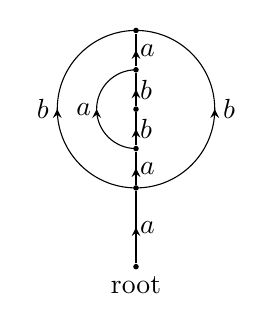
\begin{tikzpicture}[>=stealth,decoration={
				markings,
				mark=at position 0.5 with {\arrow{>}}}
	]

	\node[circle,fill=black,inner sep=0pt,minimum size=2pt] (n0) at (0,0){}node[below]{root} ;

	\node[circle,fill=black,inner sep=0pt,minimum size=2pt] (n1) at (0,1) {};
	\node[circle,fill=black,inner sep=0pt,minimum size=2pt] (n2) at (0,3) {};
  
	\draw[postaction={decorate}] (n0) --node[right=-2pt]{$a$} (n1);

  \draw[postaction={decorate},rotate=-90] (n1) arc(0:180:1); 
  \node[](n) at (1,2) {};
  \node[right=-4pt of n](m){$b$} ;

  \draw[postaction={decorate},rotate=90] (n1) arc(180:0:1);
  \node[](n) at (-1,2) {};
  \node[left=-4pt of n](m){$b$} ;

	\node[circle,fill=black,inner sep=0pt,minimum size=2pt] (i1) at (0,1.5) {};
	\node[circle,fill=black,inner sep=0pt,minimum size=2pt] (i2) at (0,2) {};
	\node[circle,fill=black,inner sep=0pt,minimum size=2pt] (i3) at (0,2.5) {};

	\draw[postaction={decorate}] (n1) --node[right=-2pt]{$a$} (i1);
	\draw[postaction={decorate}] (i1) --node[right=-2pt]{$b$} (i2);
	\draw[postaction={decorate}] (i2) --node[right=-2pt]{$b$} (i3);
	\draw[postaction={decorate}] (i3) --node[right=-2pt]{$a$} (n2);

  \draw[postaction={decorate},rotate=90] (i1) arc(180:0:0.5);
  \node[](n) at (-0.5,2) {};
  \node[left=-5pt of n](m){$a$} ;

\end{tikzpicture}
\end{document}
